    \section{Self-Composed Premier League Dataset}\label[app]{app:EPL_dataset}
        In \cref{fig:EPLdata} we present the idea behind our homemade dataset. There are in total 87 features that we use in our analysis, in addition to the actual outcome for each match.

        \begin{figure*}
            \centering
            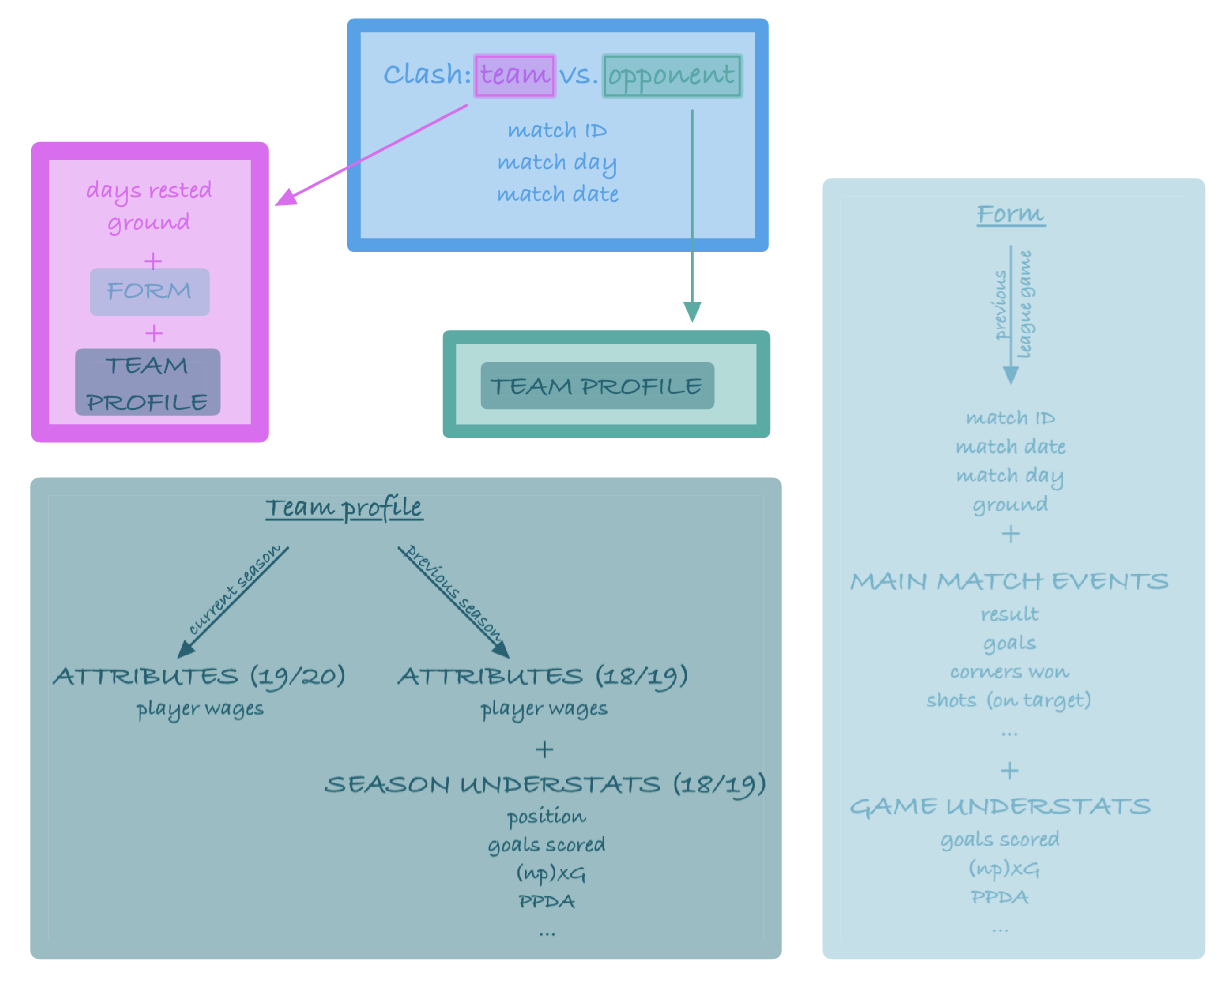
\includegraphics[width=0.78\linewidth]{figs/EPLdata_features.png}
            \caption{Schematic of how the features describing a match are connected. See text for further details.}
            \label[fig]{fig:EPLdata}
        \end{figure*}

        For a clash between a team and its opponent, we have some general facts such as what weekday it happens on and whether the team is playing on familiar ground (home) or not (away). 
        
        Both the team and the team it is facing, each have their own \textit{team profile} (lower left panel of \cref{fig:EPLdata}): information about how much the club spends on player wages\footnote{Potential to add more attributes here, such as average age and match attendance, or scope of fanbase. Extracting such data turned out to be circumstantial, which is why we have not gone further here.} from both the season we are looking at and the previous one, and a set of underlying statistics from the season before.  In addition to table position, the underlying statistics include metrics like the total xG or none-penalty xG (npxG), PPDA in the opposition half and opponent PPDA (OPPDA) in the opposition half. A number of the features describe the deviation from an estimator and the actual value, such as the difference between expected points (xpts) and actual points (pts) gained. 

        For the team we have included its form for each match, only looking back one match (again, in order to not use too much time on the data acquisition). This is why we do not include the first game week. The form (right panel of \cref{fig:EPLdata}) includes basic match data and events, as well as a set of underlying statistics somewhat larger than that of the team profile. 
    
    
    \section{Bias-variance Trade off}
        Ho ho ho! As Christmas is right around the corner, what is more tempting for both student and TA than to read two pages of extra task?! ARE YOU READY?

        We will in the following take a little detour from LWTA neural networks, to investigate an important dissection of model error. The total error of a statistical model can be decomposed into three main contributions; the \textit{bias}, \textit{variance} and \textit{irreducible} error.
        
        Every learning algorithm makes some assumptions about the relationship between the features and target output. Using a model with high bias might result in missing key relations between features and targets, frequently called underfitting. Relaxing model restrictions can yield a lower bias, but at the cost of potentially increasing the variance, often called overfitting. The variance describes how sensitive a model is to fluctuations in training data. High variance might result from a model taking training data noise into consideration when fitting its parameters. Giving the model more constraints can help to decrease the variance, at the cost of introducing more bias. This is the basis for the \textit{bias-variance tradeoff}, where we aim to find the set of parameters where both of these are small. The irreducible error comes from deviation between the assumed underlying function and the targets in the dataset (noise). As the name suggests, this contribution can not be tweaked.  
        \section{Setup and Resampling}
        We will in the following only consider regression problems \footnote{For classification problems, a similar decomposition can be performed, for instance using the \textit{Zero-One loss}, see ~\citep{zero_one_loss}}. In ~\citep{Project1} the bias-variance decomposition for the MSE was derived, giving:
        \begin{align}
            \operatorname{MSE}(\hat{f}) &= \pclosed{\bias(\hat{f})}^2 + \var(\hat{f}) + \sigma^2
        \end{align}
        With $\sigma^2$ as the irreducible error. To estimate model bias and variance, the bootstrap resampling technique will be performed, using a total of 200 bootstrap rounds for each set of model parameters. Taking different sets of models, we will compare between these and try to find the optimal model based minimizing both bias and variance. If not specified otherwise, MSE values (and of course bias and variance) is calculated using the bootstrapped test data. 

    \section{Dataset and Preparation}
        The popular video game series FIFA has new releases yearly, with a large fan base for both recreational and competitive play. Consequently, the interest of analyzing in-game data with the goal of getting a small edge is becoming more popular. For instance ~\citep{fifa21playersvalue} tries to estimate players market value based on players characteristics. Here, we will use a similar dataset ~\citep{fifa21_data}, with the goal of calculating the \textit{overall score}, a single number between 1 and 99 representing the players skill and worth. The FIFA21 version will be used. Overall score will be estimated using 38 different minor attributes, such as player dribbling skill and mental composure. All of these are real numbers in the range 1 to 99. In total there are $n = 18944$ players, where we pick a subset of $10000$ players, weighted such that we get players from different football leagues and skill levels. These $p = 38$ features are presumably not all FIFA uses to calculate the overall score, indicating that a perfect model can not be found through this approach. 
        
    \section{Umbrella term for methods not neural networks}
        We will present the key theory required for three different sets of estimation methods; \textit{Linear Regression}, \textit{Tree based methods} and \textit{Super Vector Machines}.
        \subsection{Linear Regression}
        For linear regression models, we will consider ordinary least squares (OLS), Ridge regression and Lasso regression. OLS assumes a linear relationship between the features and target, that is a specific data point is simply the sum over features, multiplied by a coefficient for each feature. Ridge and Lasso regression adds a constraint to coefficient sizes, using an $L_2$ and $L_1$ norm respectively, presumably introducing bias. This will be represented through the hyperparameter $\alpha$, proportional to the regularisation strength. See ~\citep{Project1} for a more in depth explanation.
            
        In addition, since all features are assumed to give a positive contribution to the overall score (setting all to 99 should yield an overall score of 99), the coefficients are constrained to be positive.  
        
        \subsection{Tree Based Methods}
            A decision tree uses a flow-chart like structure to generate predictions. Based on a single features value, a \textit{node} performs some test on the feature (i.e. threshold). Using the outcome of the test, the tree follows one of two paths, called \textit{branches}. Each of these branches can then have new nodes, testing based on new features, creating more branches. This continues until no more nodes are reached, where in the regression case, a specific value is predicted. These final outcomes of branches are called \textit{leaves}. The maximum number of nodes, following a single branch, gives the \textit{depth} of the tree. 
            There is a plethora of ways to construct a regression tree. The most common approach is \textit{recursive binary splitting}, where separation of the targets into regions $R_1, R_2, \ldots R_J$ is performed based on the input features. When a simple feature inequality is used, these regions are high-dimensional boxes. Considering the set of features $\set{x_a}$ $a = 1,\ldots,p$. We propose a pair of half-planes 
            \begin{align*}
                R_1(a,s) = \set{X | x_a < s} \text{ and } R_2(a,s) = \set{X | x_a \geq s}
            \end{align*}
            We then aim to find the values of $j$ and $s$ which minimizes
            \begin{align}
                \underset{a,s}{\text{argmin}}\Bigg[ \sum_{y_i \in R_1} (y_i - \bar{y}_{R_1})^2 + \sum_{y_i \in R_2} (y_i - \bar{y}_{R_2})^2 \Bigg] \label{eq:app:tree_optimasation} 
            \end{align}
            Where $\bar{y}_{R_j}$ is the calculated mean of the training data within $R_j$. This is done in a top-down approach, performing the optimasation from \cref{eq:app:tree_optimasation} down each branch, continuing until a stopping criterion is reached. This gives us our regression tree $\hat{f}(x)$, following a specific branch when evaluated for a data point $x_i$. There is no single good measure of model complexity for decision trees, but the depth gives an indication of high finely tuned predictions can become.    

            \subsubsection{Bagged Trees}
                Based on the idea of bootstrap, an ensemble of trees can be constructed. Decision trees are notorious high-variance models which are easily overfitted. By performing bootstrap resampling, a single tree can be fitted for each bag $b$, with the final prediction being the average prediction of each tree.

                \begin{align}
                    \hat{F}(x) = \frac{1}{B}\sum_{b = 1}^{B} \hat{f}^b (x) \label{eq:app:bagged_trees}
                \end{align}
                Where $\hat{f}^b$ is a single decision tree, fitted using the data from bag $b$. $B$ represents the total number of trees, which we will call ensemble size. We will call this method bagged trees (BT).

            \subsubsection{Random Forest}
                Random forest (RF) uses the same methodology as bagged trees. Bootstrap is performed in the same manner \cref{eq:app:bagged_trees}, but only a random subset of features is considered at each node split. We represent the number of features considered by $m$, with $m = 1$ reducing to bagged trees. From ~\citep{hastie01statisticallearning}, a ration of $m = \lfloor p/3 \rfloor$ usually performs well on regression problems. This is expedient since trees might be highly correlated, especially if a single feature is very important for reducing the training MSE. If all features are considered for each split, the random forest reduced to the bagged trees.
            
            \subsubsection{Boosted trees}
                The idea behind boosted trees is combining several weak learners which iteratively learn from previous mistakes to enhance performance. In the case of decision trees, weak learners are simple trees only performing slightly better than random guesses. 

                When employing gradient boost for regression the process starts by creating a single leaf, with a value $f_0(x)$ often set to the average of all output values in the training set. Implementing a differentiable cost function, e.g. the squared error for regression, the cost of the initial prediction and its gradient with respect to the predicted value is calculated. A simple tree is fitted to minimise the cost. The prediction of that tree is then scaled by a coefficient and is added to the initial prediction, $f_0(x)$, creating the next: $f_1(x) = f_0(x) + \beta b(x;\gamma_1)$. Here $\beta$ is the scaling coefficient and $\gamma_1$ the prediction parameters. The process of calculating the gradient of the cost function, fitting a new tree using the gradient, and adding this tree's prediction to the existing one, is repeated, iteratively creating a better model: 
                \begin{equation}
                    f_M(x) = f_0(x) + \sum_{m=1}^M \beta b(x; \gamma_m)
                \end{equation}
                $\beta$ can be dynamic for various $m$. In that case the gradient of the cost function must also be calculated with respect to $\beta_m$ \citep{hastie01statisticallearning}. 

        \subsection{Support Vector Machines}
            The Support Vector Machine (SVM) is most commonly used in classification problems, with the idea of constricting some hyperplane separating target classes in feature space. By a slight change of approach, the method can also be applied to regression problems, proposed in~\citep{SVR}. 
            
            \subsubsection{Regression Approach}
                The predictions are performed using a simple linear function
                \begin{align}
                    f(x_i) = \vec{w}^T x_i + b \text{ with } \vec{w} \in \mathbb{R}^p, b \in \mathbb{R} \label[eq]{eq:SVM_predict} 
                \end{align}
                We want to find the optimal values of $\set{\vec{w}, b}$ such that the predictions of $f(x_i)$ lies inside some region around the $y_i$ training data. This region is defined by the hyperparameter $\epsilon$ (the so-called $\epsilon$ intensive tube \footnote{Not to be confused with the famouse $\epsilon$-sausage used for proofs of continuity, introduced by the math professor \textit{Arne Hole}.}). This can be formulated as an optimasation of $\vec{w}$, subject to the $\epsilon$ constraint ~\citep{SVRgood}.  
                \begin{align}
                    \underset{\vec{w}}{\text{argmin  }}   ||\vec{w}||^2 
                    \hspace{10px}\text{subject to}\hspace{10px} |y_i - f(x_i)| \leq \epsilon \label[eq]{eq:SVM_optimasation}
                \end{align}
                A larger $\epsilon$ gives larger errors admitted to the solution. This is a so-called \textit{hard margin} approach, where $f(x_i)$ must make a prediction in $[y_i - \epsilon, y_i + \epsilon]$. Relaxations of this constraint can be done, allowing small deviations around the $\epsilon$ tube. This is characterized by the hyperparameter $C \geq 0$, often called a \textit{soft margin}. $C$ is proportional to the margin relaxation (inversely proportional to the regularisation strength), with $C = 0$ reducing to the hard margin approach.
            
            \subsubsection{Kernels}
                One of the benefits of SVMs is the magic of the \textit{kernel trick}. Introducing some non-linearity can improve predictions (for instance, see~\citep{Project1} for an example using linear regression). This is done by applying some transformation $\phi$ giving new features in another (often higher dimensional) space $\mathcal{F}$, $\phi: \mathbb{R}^p \xrightarrow{} \mathcal{F}$. For large data sets, especially if $\text{dim}(\mathcal{F}) \gg p$, the transformation complexity can result in long computation times. Luckily, both our model \cref{eq:SVM_predict} and optimasation \cref{eq:SVM_optimasation} only requires the computation of the dot product in $\mathcal{F}$. The kernel trick then gives us a method to calculate the transformed dot product $\phi(x_i)^T \phi(x_i)$, without explicitly calculating $\phi(x_i)$~\citep{kernelTrick}. We express this a function $K(x_i, x_j)$, witch usually some simpler dot product such as $x_i^T x_j$ or $||x_i - x_j||^2$.      
                \begin{align*}
                    \phi(x_i)^T \phi(x_j) &= K(x_i, x_j)
                \end{align*}
                In the following, we will, in addition to the linear (not transformed) product $K(x_i, x_j) = x_i^T x_j$, consider the \textit{Gaussian radial basis function} (RBF) kernel
                \begin{align}
                    \text{RBF:}\hspace{20px}& K(x_i, x_j) = \text{exp}(-\gamma ||x_i - x_j||)
                \end{align}
                Where $\gamma > 0$ is a hyperparameter. Here we will only consider $\gamma = 1/(p\sigma_X^2)$, sometimes simply called the Gaussian kernel, where $\sigma_X^2$ is the variance in $X$ across all features. 

    \section{Findings and Discussion}
        \subsection{Linear Regression}
            The bias-variance decomposition of OLS, Ridge and Lasso can be seen in figure \cref{fig:linreg_biasvar_decomp}. For OLS, there is no penalisation to vary, and all bias contributions comes from the assumption of first order polynomial response. Increasing the feature space, be it introducing higher order polynomials or exponential terms, would allow the fit to be more flexible, presumably increasing bias. When increasing the penalisation parameter $\alpha$ slightly, both Ridge and Lasso stays quite close to the simple OLS case as expected. At around $\alpha = 10^{-2}$ there is a slight decrease in both bias and variance for both models, with MSE minima at $8.46$, $8.27$ using $\alpha = 1.38, 0.12$ for Ridge and Lasso respectively. In these regions, the variance decreases as expect since the solution space for the optimal parameters shrink. There is also a dip in bias, which might be due to finding a specific set of parameters that works better for our subset of features. We do not use all of FIFAs features, as well as probably including some unimportant ones. There is probably some exclusion and inclusion bias where a penalised model better handles these by shrinking unimportant features. Going beyond the dip both Ridge and Lasso bias increases, indicating that the model is underfitting.
            \begin{figure}[H]
                \centering
                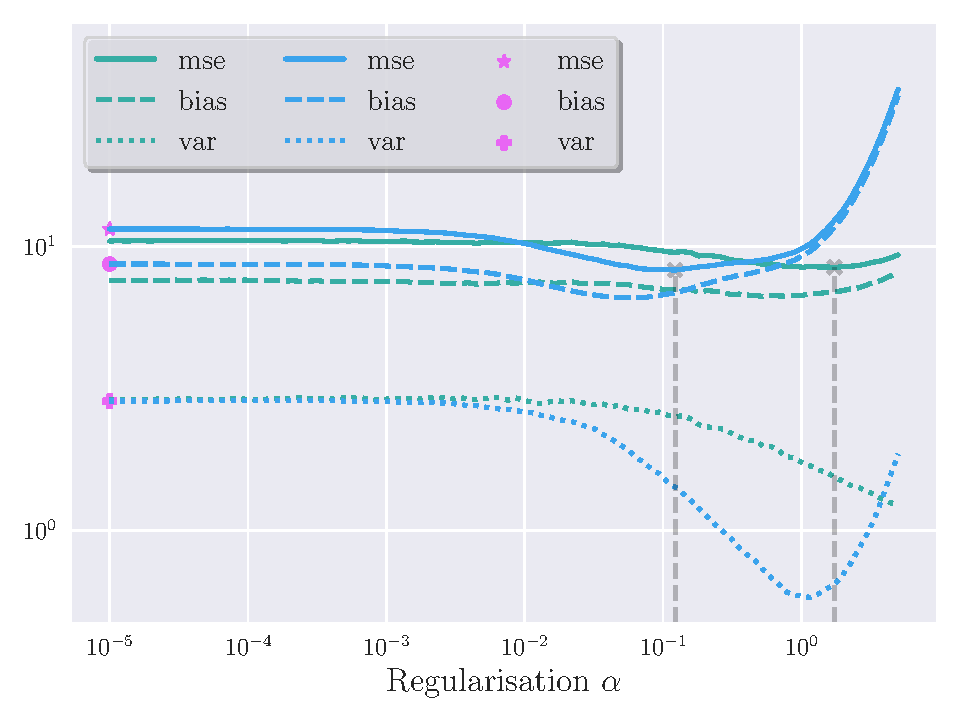
\includegraphics[width=\linewidth]{BiasVar_LinearRegression.pdf}
                \caption{MSE, bias and variance estimates for OLS (pink), Ridge (green) and Lasso (blue) as a function of regularisation parameter $\alpha$.}
                \label[fig]{fig:linreg_biasvar_decomp}
            \end{figure}

        \subsection{Tree Based Methods}
            We begin by fitting a single tree, gradually allowing for more complexity by increasing the allowed tree depth, shown in figure \cref{fig:singletree_biasvar_decomp}. In contrast to the linear regression models, the variance is significantly larger, overcoming the bias contribution for a tree of depth 2. The MSE values are generally quite large, with a minimum of $22.3$ using a depth of 2 with 4 leafs. By considering the train MSE, we see that we quickly move into the realm of extreme overfitting. Allowing the tree to grow to a depth of 5 results in close to zero train MSE. A single tree, through the parameters searched here, does not result in a good model for this problem. 
            \begin{figure}[H]
                \centering
                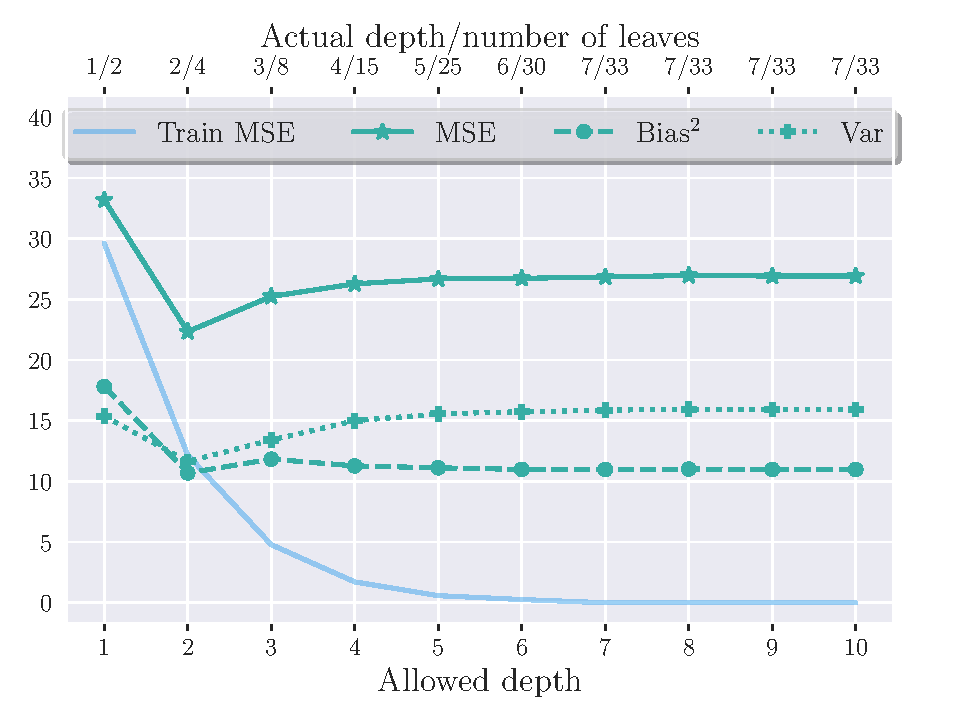
\includegraphics[width=\linewidth]{BiasVar_SingleTree.pdf}
                \caption{MSE, bias and variance estimates for a single tree against increasing relaxation of tree depth. Train MSE is also included to show the drastic overfitting.}
                \label[fig]{fig:singletree_biasvar_decomp}
            \end{figure}
            Even though a single tree did not perform well, an ensemble of trees can often give better results. Varying the number of trees in our ensemble, both the BT and RF can be seen in \cref{fig:bag_and_rf_biasvar_decomp}. Comparing with the single tree from \cref{fig:singletree_biasvar_decomp}, we see a large improvement concerning both MSE, bias and variance. When adding more trees, the variance decreases. This agrees with the idea that many high variance trees can produce a smaller variance when their predictions are averaged. Similarly, the bias decreases, but not as drastically. The rectangular distribution of targets in feature space is still assumed in this model, therefor still adding quite a lot of bias. For comparison, the bias of simple OLS from \cref{fig:linreg_biasvar_decomp} is smaller. When reaching an ensemble size of approximately $30$ trees, only slight improvements of the MSE is seen. Comparing between BT and RF, we see that considering a subset of features does decrease variance, presumably due to less correlated trees. This however does not yield significant improvements in the MSE, with BT having a more stable test MSE across different ensemble sizes than RF. 
            \begin{figure}[H]
                \centering
                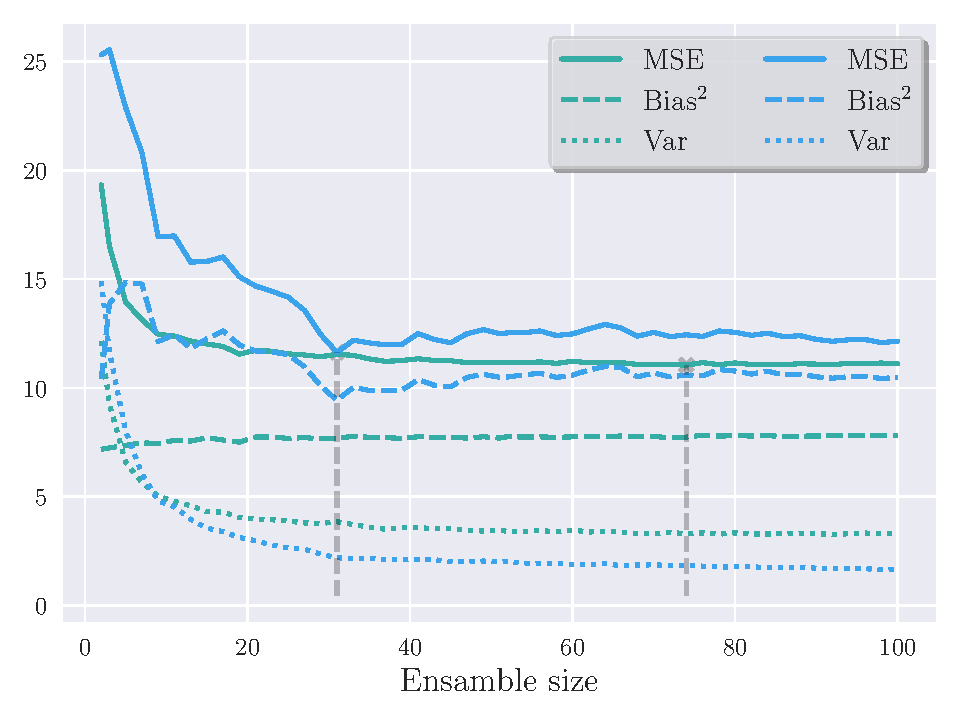
\includegraphics[width=\linewidth]{BiasVar_Bag_and_Rf.pdf}
                \caption{MSE, bias and variance estimates for bagged trees (green) and random forest (blue) considering $\lfloor p/3 \rfloor$ features as each split, against increasing bag size/number of trees.}
                \label[fig]{fig:bag_and_rf_biasvar_decomp}
            \end{figure}
            For the last of our tree based methods, we investigate the boosted trees. The MSE, bias and variance calculated while varying the number of predictors is shown in \cref{fig:boosting_n_est}. For a small ensemble size at around 10 predictors, the trees are not trained enough to give accurate score predictions, signifying that the model is underfitting. Increasing the number of predictors, the bias is decreased while the variance increases, indicating that the weak learners together has enough flexibility to mimic the underlying function. The smallest test MSE was found to be 10.89, using 17 weak learners.
            \begin{figure}[H]
                \centering
                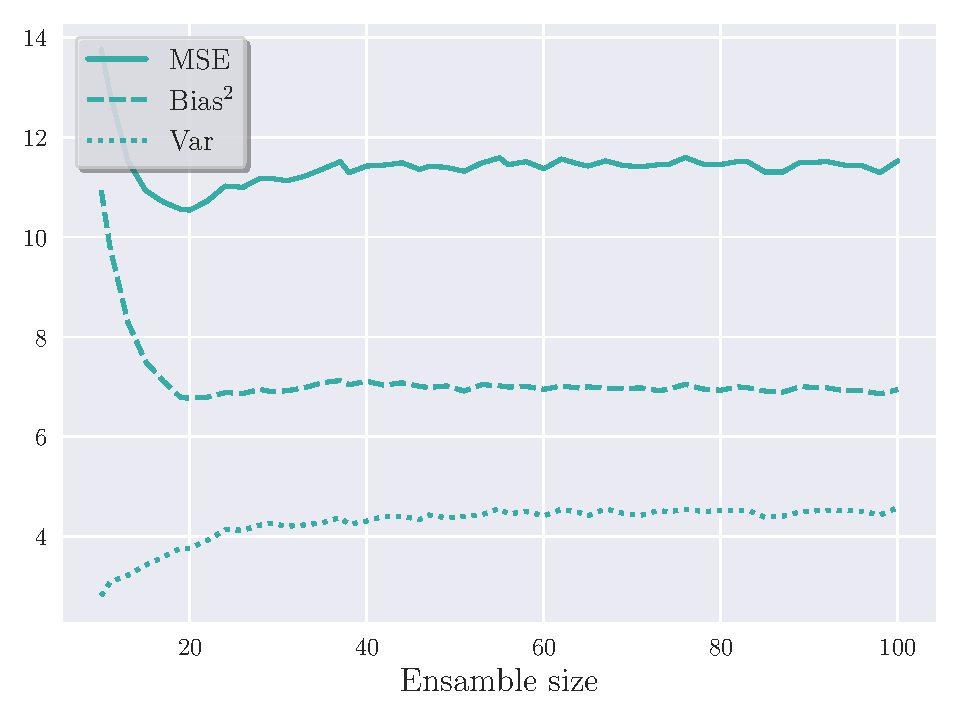
\includegraphics[width=\linewidth]{Boosting_n_est.pdf}
                \caption{MSE, bias and variance estimates for boosted trees against the increasing ensemble size.}
                \label[fig]{fig:boosting_n_est}
            \end{figure}
        
        
        \subsection{Support Vector Machines}
            Lastly, we investigate how our SVM performs when increasing the margin ($\epsilon$). To assure convergence, the margin is slightly soft, setting $C = 1$. The results from both the linear and RBF kernel can be seen in \cref{fig:SVR_eps}. For small $\epsilon$, the RBF kernel outperforms the linear kernel substantially. Though having approximately equal bias', the variance of RBF is much lower than the linear kernel. Increasing $\epsilon$ actually yields worse results for the RBF kernel, in contrast to the linear kernel where we find a low variance region with a bias dip similar to what we found for linear regression (\cref{fig:linreg_biasvar_decomp}). The increasing bias for high $\epsilon$ values might be somewhat counterintuitive, since the constraint in \cref{eq:SVM_optimasation} is loosened. However, the inclusion of many points might actually increase the bias since more points are used to center the line draw out by \cref{eq:SVM_predict}. Assuming the bagged training sample is large enough to accurately represent the population, only very small variations of the coefficients $\vec{w}$ should be allowed. This is in agreement with the variance decreasing even more for very large $\epsilon$ in \cref{fig:SVR_eps}. These results yielded optimal MSE values of $8.58$ and $11.76$ at $\epsilon = 0.35, 0.005$ for the linear and RBF kernel respectively. 

            Can we characterize bias and variance in SVMs with respect to the kernel and its parameters?
            \begin{figure}[H]
                \centering
                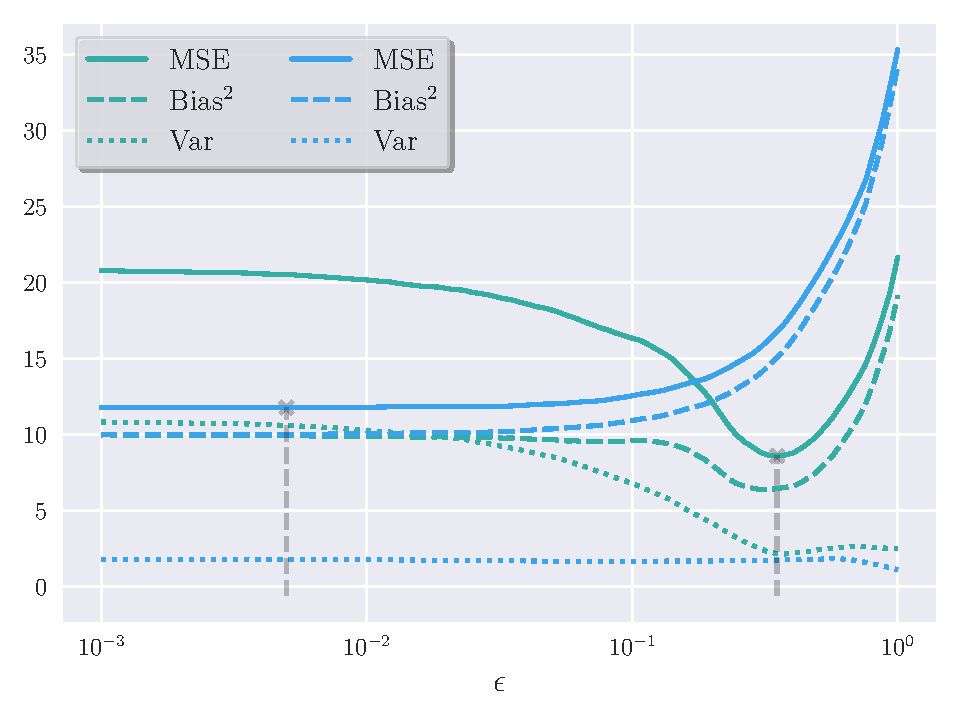
\includegraphics[width=\linewidth]{BiasVar_SVReps.pdf}
                \caption{MSE, bias and variance estimates for SVR, against increasing the margin size $\epsilon$. In green, we have the linear kernel while in blue the RBF kernel. A soft margin of $C = 1$ has been used across all $\epsilon$. }
                \label[fig]{fig:SVR_eps}
            \end{figure}
            Losning the margin, parameterised by $C$, is shown in \cref{fig:SVR_C}.
            Effects on the bias while losing the soft margin has clearer interpretation. With $C$ being small, very few or even none of the prediction by $f$ are allowed to lay outside the margin calculated by the train data. This is very clear when considering the RBF kernel, having a steeply increasing bias when $C$ approaches zero. The linear kernel however, does not seem to be very dependent on margin softness. Why this is the case is not clear, but it might give an indication of a linear $\epsilon$ tube being a good representation of the true function. However, probing the bias of different kernels is a difficult task and no obvious comparison between the two methods can be drawn. Kernel specific parameters, like $\gamma$ for RBF, can also influence the bias, see for instance~\citep{RBFkernel}. The lowest test MSE was found to be 8.25 and 10.26 at $C = 0.10, 3.77$ for the linear and RBF kernel respectively.   
            \begin{figure}[H]
                \centering
                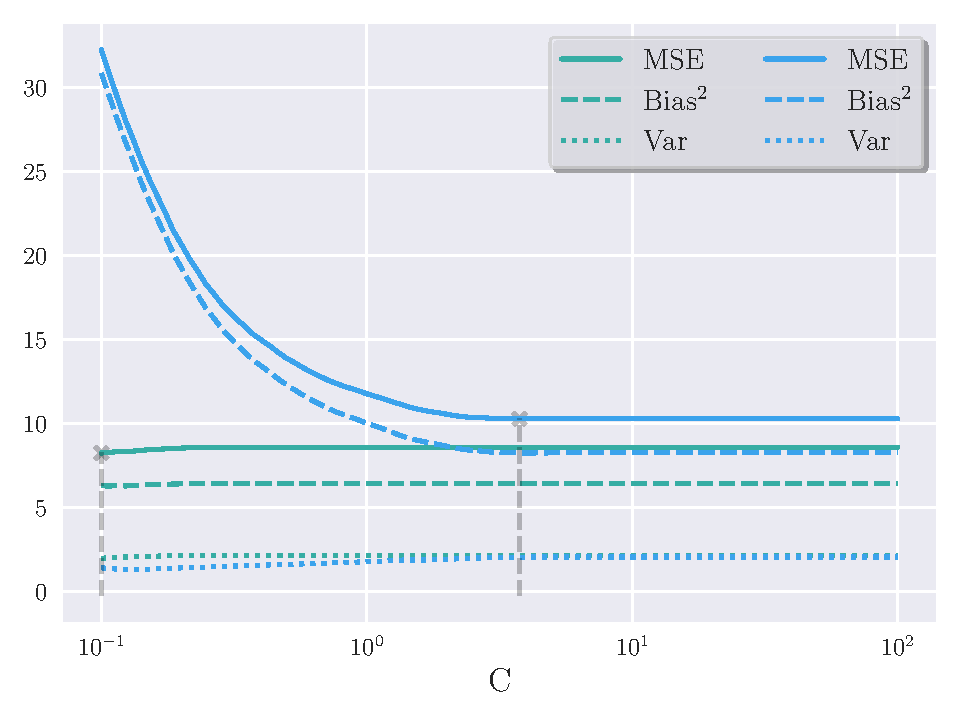
\includegraphics[width=\linewidth]{BiasVar_SVRC.pdf}
                \caption{MSE, bias and variance estimates for SVR, against increasing the softness of the margin $C$. In green, we have the linear kernel while in blue the RBF kernel. The respective optimal margin size $\epsilon$ found for $C= 1$ has been.}
                \label[fig]{fig:SVR_C}
            \end{figure}

        \subsection{Summarising Results}
            Through a study of the bootstrapped estimates for test MSE, bias and variance applied to player scores from FIFA21, we found that penalised linear regression and the linear kernel SVR performed the best. In general, the bias was larger than variance, except for the single regression tree and ensemble tree methods composed of a few trees. This is in agreement with decision trees in general being easily overfitted. Increasing the ensemble size did decrease the test MSE, with increasing variance for boosting and reducing it for BT and RF. We hypothesize that the scores calculated in FIFA21 are calculated using some linear relationship between features. Since we might have included irrelevant and excluding relevant features, the penalised linear models and linear kernel SVMs are natural choices. Moving forward, it would be interesting to make some polynomial features for the linear regression models, introducing more parameters to fit and presumably reducing bias. For SVR, more extensively searches tuning kernel parameters in addition to trying more kernels could potentially improve results. 